\documentclass[10pt,a4paper,english,landscape]{slides}

\usepackage{amsmath,amsthm,amssymb}
\usepackage{babel}
\usepackage{graphicx}
\usepackage{color}

\newcommand{\ban}{\begin{eqnarray*}}
\newcommand{\ean}{\end{eqnarray*}}
\newcommand{\ba}{\begin{eqnarray}}
\newcommand{\ea}{\end{eqnarray}}

\begin{document}


\author{Marc BARTON-SMITH\footnote{ENPC, CERMICS, } \\ \quad Jos\'e da FONSECA\footnote{INRIA Rocquencourt, Projet Mathfi}}
\title{Libor Market Model}
\date{\today}
\maketitle
\thispagestyle{myheadings}
\tableofcontents

\vspace{10mm}



\begin{center}
\fbox{{\bf Derivative products}}
\end{center}


Date structure $\lbrace T_n=T_0+n\tau ; n=1..M \rbrace $ 

assets and rates:

\begin{itemize}
\item $B(t,T)$ is the zero coupon bond at time $t$ with maturity $T$.  
\item the foward swap rate starting at date $T_s$ and ending at $T_M$ is 
\ban
S(t,T_s,T_M)=\frac{B(t,T_s)-B(t,T_M)}{\sum_{j=s+1}^{M}\tau B(t,T_j)}
\ean

\item the spot swap rate is $S(T_s,T_s,T_n)=S(T_s,T_M)$.
\item $L(t,T_i,\tau)$ the forward rate with maturity $T_i$ and length $\tau$
\end{itemize}


Arbitrage leads to  

\ba
1+\tau L(t,T_i,\tau)=\frac{B(t,T_i)}{B(t,T_{i+1})} 
\ea

spot libor rate is given by 

\ba
1+\tau L(T_i,T_i,\tau)=\frac{1}{B(T_i,T_{i+1})} 
\ea


Main products of interest for the libor Market Model

\begin{itemize}
\item Caplet and floorlet
\item Cap floor
\item swaption
\end{itemize}




\section{Libor Market Model}



Recall that 

\ban
1+\tau L(t,T_i,\tau)=\frac{B(t,T_i)}{B(t,T_{i+1})} 
\ean

and

\ban
S(t,T_s,T_M)=\frac{B(t,T_s)-B(t,T_M)}{\sum_{j=s+1}^{M}\tau B(t,T_j)}
\ean

\ban
\frac{B(t,T_i)}{B(t,T_s)}=\prod_{j=s}^{i-1}\frac{1}{1+\tau L(t,T_j,\tau)}
\ean

as such the forward swap rate as a function of the forward rates is given by the relation

\ba
S(t,T_s,T_M)=\frac{1 - \prod_{j=s}^{M-1}\frac{1}{1+\tau L(t,T_j,\tau)} }{\sum_{j=s+1}^{M}\tau \prod_{k=s}^{j-1}\frac{1}{1+\tau L(t,T_k,\tau)}} \label{tswaptfor}
\ea

In the libor market model we suppose the following dynamic for the forward Libor rates


\ban
dL(t,T_i,\tau)=L(t,T_i,\tau)\gamma(t,T_i,\tau)dW^{Q^{T_{i+1}}}
\ean

where 

\begin{itemize}
\item $\lbrace W^{Q^{T_{i+1}}}_t; t\geq 0 \rbrace$ is a $d$ dimensional brownian motion 
\item is the forward probability $Q^{T_{i+1}}$ associated with the numeraire $B(t,T_{i+1})$
\item  $\gamma(t,T_i,\tau)$ is a deterministic function. 
\item $\sigma_B(t,T)$ is the volatility of the zero coupon bond
\end{itemize}

we have the relation

\ban
\frac{\gamma(t,T_i,\tau)\tau L(t,T_i,\tau)}{1+\tau L(t,T_i,\tau)}=\sigma_B(t,T_i)-\sigma_B(t,T_{i+1})
\ean

and we deduce that

for  $i>j+1$ 

\ban
\frac{dL(t,T_j,\tau)}{L(t,T_j,\tau)}&=&\gamma(t,T_j,\tau)dW^{Q^{T_i}}_t \\
&-& \sum_{k=j+1}^{i-1}\frac{\tau L(t,T_k,\tau) \gamma(t,T_k,\tau) \gamma(t,T_j,\tau) }{1+\tau L(t,T_k,\tau)}dt
\ean

for  $j\geq i$ 

\ban
\frac{dL(t,T_j,\tau)}{L(t,T_j,\tau)}&=&\gamma(t,T_j,\tau)dW^{Q^{T_i}}_t \\
&+&\sum_{k=i}^{j}\frac{\tau L(t,T_k,\tau)\gamma(t,T_k,\tau)\gamma(t,T_j,\tau)}{1+\tau L(t,T_k,\tau)}dt
\ean


{\bf Libor market model: a stochastic volatility extension}



\begin{center}
the standart LMM is unable to fit the smile 

$\Downarrow$

a stochastic volatility extension 
\end{center}



{\it The model}

Under the risk neutral measure $Q$ the zero coupon bond follows the dynamic

\ban
\frac{dB(t,T)}{B(t,T)}&=&r(t)dt+\sqrt{V_t}\sigma_B(t,T)'dW_t\\
dV_t&=&\kappa(\theta - V_t)dt+\epsilon \sqrt{V_t}dZ_t
\ean

where 

\begin{itemize}
\item $\left( W_t;t\geq 0 \right)$ is a $d$ dimensional brownian motion under $Q$
\item $\left( Z_t;t\geq 0 \right)$ is a $1$ dimensional brownian motion under $Q$, 
\item $\sigma_B(t,T)$ is a $1*d$ vector
\end{itemize}

we have 

\ban
\frac{dL(t,T_j,\tau)}{L(t,T_j,\tau)}&=&\sqrt{V_t}\gamma(t,T_j,\tau)'[dW^Q_t-\sqrt{V_t}\sigma_B(t,T_{j+1})dt] \\
dV_t&=&\kappa(\theta - V_t)dt+\epsilon \sqrt{V_t}dZ_t
\ean

with

\ba
\gamma(t,T_j,\tau)=\frac{1+\tau L(t,T_j,\tau)}{\tau L(t,T_j,\tau)}[\sigma_B(t,T_j)-\sigma_B(t,T_{j+1})] \label{forwardvolbondvol}
\ea


we make the hypothesis  

\begin{center}
\fbox{ $\lbrace \gamma(t,T_j,\tau) ; \; t \geq 0 ;\; j=1..M \rbrace $ are deterministic functions. }
\end{center}


We note $\gamma(t,T_j,\tau)=(\gamma^1(t,T_j,\tau),\gamma^2(t,T_j,\tau),..,\gamma^d(t,T_j,\tau) )$ \\

From (\ref{forwardvolbondvol}) and under the hypothesis $\sigma_B(t,T_1)=0$ we obtain

\ban
\sigma_B(t,T_{j+1})=-\sum_{k=1}^j\frac{1+\tau L(t,T_j,\tau)}{\tau L(t,T_j,\tau)}\gamma(t,T_k,\tau) 
\ean

correlation between the forward rate factors and the volatility factor:

\ban
\frac{\gamma(t,T_j,\tau)'dW_t}{||\gamma(t,T_j,\tau)||}dZ_t=\rho_j(t)dt
\ean

If we note $W_t=(W^1_t,..,W^d_t)$ and $dW^i_tdZ_t=\rho^idt$ we have 

\ba
||\gamma(t,T_j,\tau)||\rho_j(t)dt&=& \gamma(t,T_j,\tau)'dW_tdZ_t\\
&=&\sum_{i=1}^d \rho^i\gamma^i(t,T_j,\tau) dt \label{rhovol}
\ea



under  $Q^{T_{j+1}}$ the probability measure associated with $B(t,T_{j+1})$  as numeraire  we have

\[
\left\lbrace 
\begin{array}{l}
\frac{dL(t,T_j,\tau)}{L(t,T_j,\tau)}=\sqrt{V_t}\gamma(t,T_j,\tau)'dW^{Q^{T_{j+1}}}_t \\
dV_t=\kappa(\theta - (1+\frac{\epsilon}{\kappa}\xi_j(t))V_t)dt+\epsilon \sqrt{V_t}dZ^{Q^{T_{j+1}}}_t
\end{array}
\right.
\]

where $W^{Q^{T_{j+1}}}_t$ resp. $Z^{Q^{T_{j+1}}}_t$ is a $1*d$ resp. $1$ dimensional brownian motion under $Q^{T_{j+1}}$ and 

\ban
\xi_j(t)=\sum_{k=1}^j\frac{\tau L(t,T_k,\tau)}{1+\tau L(t,T_k,\tau)}\rho_k(t)||\gamma(t,T_k,\tau)|| 
\ean

the authors propose to freeze this stochastic process and  define 

\ban
\xi_j^0(t)=\sum_{k=1}^j\frac{\tau L(0,T_k,\tau)}{1+\tau L(0,T_k,\tau)}\rho_k(t)||\gamma(t,T_k,\tau)|| 
\ean

\ban
\tilde \xi_j(t)&=&1+\frac{\epsilon}{\kappa} \xi_j(t)\\
\tilde \xi_j^0(t)&=&1+\frac{\epsilon}{\kappa}\xi_j^0(t)
\ean

thus the dynamic is given by

\[
\left\lbrace 
\begin{array}{l}
\frac{dL(t,T_j,\tau)}{L(t,T_j,\tau)}=\sqrt{V_t}\gamma(t,T_j,\tau)'dW^{Q^{T_{j+1}}}_t \\
dV_t=\kappa(\theta - \tilde \xi_j^0(t)V_t)dt+\epsilon \sqrt{V_t}dZ^{Q^{T_{j+1}}}_t
\end{array}
\right.
\]

{\bf Moment generating function for the caplet}

Computing the moment generating function for $X_u=ln \frac{L(u,T_j,\tau)}{L(t,T_j,\tau)}$ , define 

\ban
\phi(t,X_t,V_t,z)=E^{Q^{T_{j+1}}}\left[ e^{zX_{T_j}}|{\cal F}_t \right]
\ean

The function $\phi(t,x,V,z)$ satisfies the pde

\[
\left\lbrace 
\begin{array}{l}
\partial_t\phi+\kappa(\theta - \tilde \xi_j^0(t)V)\partial_V\phi -\frac{1}{2}||\gamma(t,T_j,\tau)||^2V\partial_x\phi \\
+\frac{1}{2}\epsilon^2V\partial^2_{VV}\phi+\epsilon\rho_j(t)V||\gamma(t,T_j,\tau)||\partial^2_{Vx}\phi+\frac{1}{2}||\gamma(t,T_j,\tau)||^2V\partial^2_{xx}\phi=0\\
\phi(T,x,V,z)=e^{zx}
\end{array}
\right.
\]



we define the function 

\ba
\phi_T(z)=\phi(t,0,V_t,z) \label{fi0}
\ea


{\bf Moment generating function for the swaption}

For the swaption pricing: recall 

\ban
S(t,T_s,T_M)&=&\frac{B(t,T_s)-B(t,T_M)}{\sum_{j=s+1}^{M}\tau B(t,T_j)}\\
&=&\frac{1 - \prod_{j=s}^{M-1}\frac{1}{1+\tau L(t,T_j,\tau)} }{\sum_{j=s+1}^{M}\tau \prod_{k=0}^{j-1}\frac{1}{1+\tau L(t,T_k,\tau)}}
\ean

using Ito's lemma we deduce that 

\ban
dS(t,T_s,T_M)&=&\sum_{j=s}^{M-1}\frac{\partial S(t,T_s,T_M) }{\partial L(t,T_j,\tau)}L(t,T_j,\tau)\sqrt{V_t}\gamma(t,T_j,\tau)'\\
& &[dW_t-\sqrt{V_t}\sigma_S(t)dt]\\
dV_t&=&\kappa(\theta - \tilde \xi_S(t)V_t)dt+\epsilon \sqrt{V_t}[dZ_t+\xi_S(t)dt]
\ean

with

\ban
\sigma_S(t)&=&\sum_{j=s}^{M-1}\alpha_j(t)\sigma_B(t,T_{j+1})\\
\tilde \xi_S(t)&=&1+\frac{\epsilon}{\kappa}\sum_{j=s}^{M-1}\alpha_j(t)\xi_j(t)\\
\alpha_j(t)&=&\frac{\tau B(t,T_{j+1})}{ \sum_{j=s}^{M-1} \tau B(t,T_{j+1})}\\
\frac{\partial S(t,T_s,T_M) }{\partial L(t,T_j,\tau)}&=&\frac{\tau S(t,T_s,T_M)}{(1+\tau L(t,T_j,\tau))}\\
&&\left( \frac{B(t,T_M)}{B(t,T_s)-B(t,T_M)}+\frac{\sum_{k=j+1}^M \tau B(t,T_k)}{\sum_{j=s+1}^{M}\tau B(t,T_j)}  \right)
\ean

the dynamic of the forward swap rate is given by

\[
\left\lbrace 
\begin{array}{l}
dS(t,T_s,T_M)=\sum_{j=s}^{M-1}\frac{\partial S(t,T_s,T_M) }{\partial L(t,T_j,\tau)}L(t,T_j,\tau)\sqrt{V_t}\gamma(t,T_j,\tau)'dW^{Q^S}_t\\
dV_t=\kappa(\theta - \tilde \xi_S(t)V_t)dt+\epsilon \sqrt{V_t}dZ^{Q^S}_t
\end{array}
\right.
\]

with

\ban
dW^{Q^S}_t&=&dW_t-\sqrt{V_t}\sigma_S(t)dt\\
dZ^{Q^S}_t&=&dZ_t-\sqrt{V_t}\xi_S(t)dt
\ean

where $W^{Q^S}_t$ resp. $Z^{Q^S}_t$ is a $1*d$ dimensional resp $1$ dimensionnal brownian motion under $Q^S$.

 
freezing the volatility for the forward swap rate and the drift of the volatility we get


\[
\left\lbrace 
\begin{array}{l}
\frac{dS(t,T_s,T_M)}{S(t,T_s,T_M)}= \sum_{j=s}^{M-1}\omega_j(0)\sqrt{V_t}\gamma(t,T_j,\tau)'dW^{Q^S}_t\\
dV_t=\kappa(\theta - \tilde \xi_S^0(t)V_t)dt+\epsilon \sqrt{V_t}dZ^{Q^S}_t
\end{array}
\right.
\]

\ban
\omega_j(0)&=&\frac{\partial S(0,T_s,T_M) }{\partial L(0,T_j,\tau)}\frac{L(0,T_j,\tau)}{S(0,T_s,T_M)}\\
\tilde \xi_S^0(t)&=&1+\frac{\epsilon}{\kappa}\sum_{j=s}^{M-1}\alpha_j(0)\xi_j^0(t)
\ean

Computing the moment generating function for $X_u=ln\frac{S(u,T_s,T_M)}{S(t,T_s,T_M)}$ , define 

\ban
\phi(t,X_t,V_t,z)=E^{Q^S}\left[ e^{zX_T}|{\cal F}_t\right]
\ean

The function $\phi(t,x,V,z)$ satisfies the pde

\[
\left\lbrace 
\begin{array}{l}
\partial_t\phi+\kappa(\theta - \tilde \xi_S^0(t)V)\partial_V\phi -\frac{1}{2}||\gamma_{s,M}(t)||^2V\partial_x\phi \\
+\frac{1}{2}\epsilon^2V\partial^2_{VV}\phi+\epsilon\rho^S(t)V||\gamma_{s,M}(t)||\partial^2_{Vx}\phi+\frac{1}{2}||\gamma_{s,M}(t)||^2V\partial^2_{xx}\phi=0\\
\phi(T,x,V,z)=e^{zx}
\end{array}
\right.
\]

with

\ban
\gamma_{s,M}(t)&=&\sum_{j=s}^{M-1}\omega_j(0)\gamma(t,T_j,\tau)\\
\rho^S(t)&=&\frac{\sum_{j=s}^{M-1} \omega_j(0)||\gamma(t,T_j,\tau)||\rho_j(t) }{||\gamma_{s,M}(t)||}
\ean

furthermore the authors suggest, arguing a calibration objective not presented in the paper, to approximate

\ban
\rho^S(t)\sim\sum_{j=s}^{M-1}\omega_j(0)\rho_j(t)
\ean
 
In fact, this approximation is useless because only  $\rho^S(t)||\gamma_{s,M}(t)||$ is needed and (\ref{rhovol}) is used.


We define the function $\phi_T(z)$ by 

\ba
\phi_T(z)=\phi(t,0,V_t,z) \label{fi1}
\ea


{\bf Computing the moment generating function}

The pdes are identical as such we write both in a compact form

\[
\left\lbrace 
\begin{array}{l}
\partial_t\phi  +\kappa(\theta - \beta(t)V)\partial_V\phi -\frac{1}{2}\lambda(t)^2V\partial_x\phi\\
+\frac{1}{2}\epsilon^2V\partial^2_{VV}\phi+\epsilon\rho(t)V\lambda(t)\partial^2_{Vx}\phi+\frac{1}{2}\lambda(t)^2V\partial^2_{xx}\phi=0\\
\phi(T,x,V,z)=e^{zx} 
\end{array}
\right. 
\]


for the caplet

\ban
\beta(t)&=& \tilde \xi_j^0(t) \\
\lambda(t)&=&||\gamma(t,T_j,\tau)|| \\
\rho(t)&=&\rho_j(t)\\
\zeta(t)&=&||\gamma(t,T_j,\tau)||  \rho_j(t)
\ean


for the swaption

\ban
\beta(t) &=& \tilde \xi_S^0(t)\\
\lambda(t) &=& ||\gamma_{s,M}(t)|| \\
\rho(t) &=& \rho^S(t)\\
\zeta(t)&=&\rho^S(t)||\gamma_{s,M}(t)|| 
\ean

we emphazis the time dependence of the parameters. Looking for a solution of the form $\phi(t,x,V,z)=e^{A(t,z)+B(t,z)V+zx}$ we obtain the Riccati's equations

\ba
-\partial_tA(t,z)&=&\kappa \theta B(t,z)\\
-\partial_tB(t,z)&=&\frac{1}{2}\epsilon^2B(t,z)^2+(\rho(t)\epsilon\lambda(t)z-\kappa\beta(t) )B(t,z)+\frac{1}{2}\lambda(t)^2(z^2-z)\\ \label{riccati1}
&=&b_2(t)B(t,z)^2+b_1(t)B(t,z)+b_0(t)
\ea

with terminal conditions $A(T,z)=0$ and $B(T,z)=0$


Under the hypothesis that the volatility is piecewise constant and the maturity of the option is $T_N$ the solution of the above system is given by

\[
\left\lbrace 
\begin{array}{l}
B(t,z)=B(T_{i+1},z)+\frac{-b_1+d-2B(T_{i+1},z)b_2}{2b_2(1-ge^{d(T_{i+1}-t)})}(1-e^{d(T_{i+1}-t)})\\
A(t,z)=A(T_{i+1},z)+\frac{a_0}{2b_2}\left(  (-b_1+d)(T_{i+1}-t)-2ln\left(\frac{1-ge^{d(T_{i+1}-t)}}{1-g} \right)   \right)
\end{array}
\right. 
\]

for $t\in [T_i\; T_{i+1}]$ and $i \in \lbrace 0..N-1 \rbrace $ with 

\ban
A(T_N,z)&=&0\\
B(T_N,z)&=&0\\
a_0&=&\kappa \theta\\
b_1&=&\rho(T_i) \epsilon \lambda(T_i) z -\kappa \beta(T_i) \\
b_0&=&\frac{\lambda(T_i)^2}{2}(z^2-z)\\
b_2&=&\frac{\epsilon^2}{2}\\
d&=&\sqrt{\Delta}\\
\Delta&=&b_1^2-4b_0b_2\\
g&=&\frac{-b_1+d -2 B(T_{i+1},z)b_2}{-b_1-d -2 B(T_{i+1},z)b_2} 
\ean


{\bf Remark}: For computational prupose we embed the caplet/floorlet structure in the swpation structure. In fact we have


\ban
L(t,T_i,\tau)=S(t,T_i,T_{i+1})
\ean

as such for pricing a caplet or a swaption we will use the same algorithm.

{\bf Derivatives pricing}

For the caplet $Cplt(t,T_M,K,\tau,N)$ we have

\ban
Cplt(t,T_M,K,\tau,N)&=&B(t,T_M+\tau)\tau N E^{Q^{T_M+\tau}}_t[(L(T_M,T_M,\tau)-K)_+]\\
&=&B(t,T_M+\tau)\tau N L(t,T_M,\tau) \left( I_1 - \frac{K}{L(t,T_M,\tau)}I_2 \right)
\ean

with

\ban
I_1&=&E^{Q^{T_M+\tau }}_t\left[ e^{ln\frac{L(T_M,T_M,\tau)}{L(t,T_M,\tau)}} {\bf 1}_{\lbrace \frac{L(T_M,T_M,\tau)}{L(t,T_M,\tau)}>\frac{K}{L(t,T_M,\tau)} \rbrace } \right]\\
I_2&=&E^{Q^{T_M+\tau }}_t\left[  {\bf 1}_{ \lbrace \frac{L(T_M,T_M,\tau)}{L(t,T_M,\tau)}>\frac{K}{L(t,T_M,\tau)} \rbrace }\right]
\ean



For the floorlet $Flt(t,T_M,K,\tau,N)$ we have

\ban
Flt(t,T_M,K,\tau,N)&=&B(t,T_M+\tau)\tau N L(t,T_M,\tau)\\
& &\left( (1-I_2)\frac{K}{L(t,T_M,\tau)} -(1-I_1) \right)
\ean

For the european payer  swaption $Swpt(t,T_s,T_M,K,\tau,N)$ 

\ban
Swpt(t,T_s,T_M,K,\tau,N)&=& \sum_{i=s}^{M-1} B(t,T_{i+1}) \tau N S(t,T_s,T_M) \\
&&\left( I_1 - \frac{K}{S(t,T_s,T_M)}I_2 \right)
\ean

\ban
I_1&=&E^{Q^S}_t\left[ e^{ln\frac{S(T_s,T_s,T_M)}{S(t,T_s,T_M)}} {\bf 1}_{\lbrace \frac{S(T_s,T_s,T_M)}{S(t,T_s,T_M)}>\frac{K}{S(t,T_s,T_M)} \rbrace } \right]\\
I_2&=&E^{Q^S}_t\left[  {\bf 1}_{ \lbrace \frac{S(T_s,T_s,T_M)}{S(t,T_s,T_M)}>\frac{K}{S(t,T_s,T_M)} \rbrace }\right]
\ean

For the  european receiver swaption $Swpt(t,T_s,T_M,K,\tau,N)$ 

\ban
Swpt(t,T_s,T_M,K,\tau,N)&=& \sum_{i=s}^{M-1} \tau B(t,T_{i+1}) N S(t,T_s,T_M) \\
&&\left( \frac{K}{S(t,T_s,T_M)}(1-I_2) - (1-I_2) \right) 
\ean



{\bf Computing the integrals}


We have the following expressions for $I_1$ and $I_2$



\ban
I_1&=&\frac{1}{2}+\frac{1}{\pi}\int_0^{+\infty} \frac{ Im\lbrace e^{-iuln\left( \frac{K}{X(t)} \right)}   \phi_T(1+iu) \rbrace }{u}du\\
I_2&=&\frac{1}{2}+\frac{1}{\pi}\int_0^{+\infty} \frac{ Im\lbrace e^{-iuln\left( \frac{K}{X(t)} \right) }   \phi_T(iu) \rbrace }{u}du
\ean

where $\phi_T(u)$ is given by (\ref{fi0}) or (\ref{fi1}) depending on whether a swaption or a caplet is priced and $X(t)=L(t,T_M,\tau)$ resp. $X(t)=S(t,T_s,T_M)$ for the caplet/floorlet resp. the swaption (receiver or payer). 
\\
FFT method is also possible




{\bf Numerical examples} 

For our numerical experiments we choose a two factors model with the following piecewise volatility structure: 

$\gamma(t,T_k,\tau)=(\gamma^1(t,T_k,\tau),\gamma^2(t,T_k,\tau))$.  


if $t\in [T_j \; T_{j+1}[$ 

\ban
\gamma^1(t,T_k,\tau)&=&0.2\\
\gamma^2(t,T_k,\tau)&=& \frac{0.01-0.05e^{-0.1(j-k)}}{\sqrt{0.04+0.00075j}}
\ean

and 

\ban
dW^1_tdZ_t&=&\rho^1dt=0.5 dt\\
dW^2_tdZ_t&=&\rho^2dt=0.2 dt
\ean

the yield curve is flat at $5\%$, $V_0=1$, $\epsilon=0.6$, $\kappa=1$ and $\theta=1$.
\begin{center}
{\bf Swaption payer prices in bps}\\
\begin{tabular}{|cccc|}\hline
{\small swaption maturity}  & Tenor     & strike      &   price   \\ \hline
  1      &  1    &    ATM   &  64.519   \\  
  1      &  5    &    ATM   &  405.221    \\
  1      &  10   &    ATM   &  1179.612    \\
  3      &  1    &    ATM   &  116.830   \\  
  3      &  5    &    ATM   &  739.835    \\
  3      &  10   &    ATM   &  2057.297     \\
  5      &  1    &    ATM   &   161.735  \\  
  5      &  5    &    ATM   &   1009.870 \\
  5      &  10   &    ATM   &   1904.210  \\ \hline
  1      &  1    &    0.8 ATM   &   114.683  \\  
  1      &  5    &    0.8 ATM   &    609.080 \\
  1      &  10   &    0.8 ATM   &    1472.062  \\
  3      &  1    &    0.8 ATM   &    151.380 \\  
  3      &  5    &    0.8 ATM   &    869.485 \\
  3      &  10   &    0.8 ATM   &    2201.807  \\
  5      &  1    &    0.8 ATM   &    185.766 \\  
  5      &  5    &    0.8 ATM   &    1087.164 \\
  5      &  10   &    0.8 ATM   &    2257.460  \\ \hline
\end{tabular} 
\end{center} 


\begin{center}
{\bf Swaption payer prices in bps}\\
\begin{tabular}{|cccc|}\hline
{\small swaption maturity}  & Tenor     & strike      &   price   \\ \hline
  1      &  1    &    1.2 ATM   &    34.655 \\  
  1      &  5    &    1.2 ATM   &    267.585 \\
  1      &  10   &    1.2 ATM   &    954.980  \\
  3      &  1    &    1.2 ATM   &    91.083 \\  
  3      &  5    &    1.2 ATM   &    636.496 \\
  3      &  10   &    1.2 ATM   &    1934.698  \\
  5      &  1    &    1.2 ATM   &    142.306  \\  
  5      &  5    &    1.2 ATM   &    944.592 \\
  5      &  10   &    1.2 ATM   &    1623.445  \\ \hline
\end{tabular} 
\end{center} 

\newpage
%%\section{Arbitrage free discretization of the Libor Market Model}

{\bf Arbitrage free discretization of the Libor Market Model}

\subsection{Definition of {\it arbirtrage-free} discretization}

In the BGM models it is supposed that all the libor $L(t,T_i,\tau)$ under their own forward measure $Q^{T_{i+1}}$  has no drift and 
deterministic log-volatility :
$$\forall i=1,..,M : \quad dL(t,T_i,\tau)=L(t,T_i,\tau)\gamma_i(t).dW^{Q^{T_{i+1}}}_t.$$
Considering a numeraire $N(t)$, we denote by $D_i$ the deflated bonds :
$$\forall i=1,..,M+1 : D_i(t)=\frac{B(t,T_i)}{N(t)}.$$

\noindent By definition of a numeraire the deflated bonds are martingale under their corresponding measure $Q^N$ associated to the numeraire $N$.
This martingale property is of course for the continuous filtration.\\
The deflated bonds price can be defined by the libors :
$$\forall t<T_i:\quad D_i(t)=\frac{B(t,T_{i_t})}{N(t)}\prod_{j=i_t}^{i-1}\frac{1}{1+\tau
    L(t,T_j,\tau)},\quad \hbox{for } i=i_t,..,M+1$$
where $i_t$ is the unique integer such that $T_{i_t-1} \le t
<T_{i_t}$.\\

\noindent {\bf Definition :} A discretisation $0=t_0<t_1<...<t_n=T_{M+1}$ is said to be
{\it arbitrage-free} if all the discrete deflated bonds are discrete
martingale. In other words, if we denote $\hat{D_i}(t_j)$ the computed
deflated bond $D_i$ in time $t_j$, we must have :
\begin{equation}
\label{def}
\forall i=1,..,M+1, \quad j=0,..,n-1
:\hat{D_i}(t_j)=E\left[\hat{D_i}(t_{j+1}) _{/{F}_j}\right]
\end{equation}
where ${F}_j$ is the filtration  associed to the discrete brownian
process over ${t_0, t_1, ...,t_n}$.\\

\noindent {\bf Remark :} Thus the condition to an {\it arbitrage-free}
discretisation can be resumed to these backward discrete relations.

\subsection{Two usefull numeraires for {\it arbitrage-free}}
There are two numeraires that will be usefull to seek {\it
  arbitrage-free} dicretization.\\
the terminal numeraire :
$$N_T(t)=B(t,T_{M+1})$$
and the spot numraire ($i_t$ such that: $T_{i_t-1} \le t<T_{i_t}$):
$$N_S(t)=\frac{B(t,T_{i_t})}{B(0,T_1) \prod_{j=1}^{i_t-1}B(T_j,T_{j+1})}$$

Both numeraires have the great advantage, for a libor model, to give the
expression of the deflated bonds  only with respect to the libors :
\ba
\label{DtfL}
D_i(t)&=&\prod_{j=i}^{M}\left(1+\tau L(t,T_j,\tau)\right)\quad
\hbox{for the terminal numeraire}\\
\label{DsfL}
D_i(t)&=&B(0,T_1)\prod_{j=1}^{i-1}\frac{1}{1+\tau L(t,T_j,\tau)}\quad
\hbox{for the spot numeraire}
\ea
for all $i=1,...,M+1$.\\
Thus in the {\it libors discrete world}, denoting for all $i=0,..,n$
and $j=1,..,M$
$\hat{L}(t_i,T_j,\tau)$ the numerical computed value of the
libors, the discrete deflated bonds price are: 
\ba
\hat{D}_i(t)&=&\prod_{j=i}^{M}\left(1+\tau \hat{L}(t,T_j,\tau)\right)\quad
\hbox{for the terminal numeraire}\\
\hat{D}_i(t)&=&B(0,T_1)\prod_{j=1}^{i-1}\frac{1}{1+\tau \hat{L}(t,T_j,\tau)}\quad
\hbox{for the spot numeraire}
\ea
\subsection{Continuous martingales versus discrete Martingale}
\begin{itemize}
\item Martingale property of the continuous deflated bonds does not imply the martingale property of the discrete deflated bonds
\item in a BGM model the libors $\hat{L}_i$ or log-libors $log(\hat{L}_i)$ are computed through a standart Euler scheme then the $\hat{D}_i$ have no (discrete) martingale
\end{itemize}

Main strategy to solve this problem:



\begin{center}
Other assets associated to the libors by a bijective relation will be discretized to make the {\it arbitrage-free} discretisation true

$\Downarrow$

that is to say to make the discrete deflated bonds martingale.
\end{center}

Two assets that can be considered: $X$ and $Y$ given by :

\ba
\label{XfL}
X_i(t)&=&L(t,T_i,\tau)\prod_{j=i+1}^{M}\left(1+\tau
  {L}(t,T_j,\tau)\right) \quad \forall i=1,..,M.\\
\label{YfL}
Y_i(t)&=&\tau L(t,T_i,\tau)\prod_{j=1}^{i}\frac{1}{1+\tau
  {L}(t,T_j,\tau)} \quad \forall i=1,..,M.
\ea

Taking $Y_{M+1}(t)=\prod_{j=1}^{M}\frac{1}{1+\tau   \hat{L}(t,T_j,\tau)}$ we have the following equalities:

\begin{equation}
\sum_{j=1}^{M+1} Y_j(t) = 1.
\end{equation}

The libors can aslo be written with respect to this assets :

\ba
\label{LfX}
L_i(t,T_i,\tau)&=&\frac{X_i(t)}{1+\tau X_{i+1}(t)+..+\tau X_M(t)} \quad \forall i=1,2,..,M.\\
\label{LfY}
L_i(t,T_i,\tau)&=&\frac{Y_i(t)}{\tau (Y_{i+1}(t)+..+Y_{M+1}(t))} \quad \forall i=1,2,..,M.
\ea

The deflated bonds  can also be written with respect to these assets :

\ba
\label{DtfX}
D_i(t)&=&1+\tau \sum_{j=i}^{M}X_j(t) \quad \hbox{for terminal numeraire}\\
\label{DsfY}
D_i(t)&=&B(0,T_1)\sum_{j=i}^{M+1}Y_j(t) \quad \hbox{for spot numeraire}
\ea

and vice versa :

\ba
\label{XfD}
X_i(t)&=&\frac{1}{\tau}(D_i(t)-D_{i+1}(t)) \quad \hbox{for terminal numeraire}\\
\label{YfD}
Y_i(t)&=& \frac{D_i(t)-D_{i+1}(t)}{B(0,T_1)}\quad \hbox{for spot numeraire}
\ea

{\it Theorem:} The assets $X$ and $Y$ are martingale respectively under the terminal and spot measure.\\


{\it Theorem:} Under their measure the EDS verified by $X$ and $Y$ are the following~:

\ba
\frac{dX_i(t)}{X_i(t)}&=&\left( \gamma_i(t) + \sum_{j=i+1}^M\frac{\tau 
    X_j(t)*\gamma_j}{1+\tau X_j(t)+...+\tau X_M(t)} \right).dW^{Q^{N_T}} \quad \forall i=1,..,M.\\
\frac{dY_i(t)}{Y_i}&=& \left(\gamma_i
+\sum_{i_t}^{i}\frac{Y_j *\gamma_j}{Y_{j-1}+..+Y_1-1}\right).dW^{Q^{N_S}} \quad
\forall i=1,..,M+1.
\ea


{\bf Implementation of caps and swaptions with $X$ and $Y$}

{\it Theorem} With a standart log Euler scheme, the discrete assets $\hat{X}$ and $\hat{Y}$ are discrete martingales.


\noindent Considering a receiver swaption of a swap rate between $T_\alpha$ and
$T_\beta$ ($\alpha<\beta<M+1$), under the numeraire measure $Q^N$ we
have for its price at time $t=0$ :

\ba
\frac{RS_{\alpha,\beta}}{N(0)}&=&E\left[\frac{1}{N(T_\alpha)}\left(1-B(T_\alpha,T_\beta)-K\sum_{j=\alpha+1}^\beta
    \tau B(T_\alpha,T_j)\right)\right]\\
\label{RS}
\frac{RS_{\alpha,\beta}}{N(0)}&=&E\left[D_\alpha(T_\alpha)-D_\beta(T_\alpha)-K\tau\sum_{j=\alpha+1}^\beta
  D_j(T_\alpha)\right]
\ea

\noindent {\bf Swaption price for asset $X$} :
With equality (\ref{DtfX}) in (\ref{RS}) we get under terminal measure :

\begin{equation}
\frac{RS_{\alpha,\beta}}{B(0,T_{M+1})}=\tau E\left[ \sum_{j=\alpha}^{\beta-1}
  X_j(T_\alpha) - K\tau \sum_{j=\alpha+1}^\beta \left(1+\tau
    \sum_{k=j}^M X_k(T_\alpha)\right)\right]
\end{equation}

\noindent {\bf Swaption price for asset $Y$} :  
With equality (\ref{DsfY}) in (\ref{RS}) we get under spot measure:

\begin{equation}
\frac{RS_{\alpha,\beta}}{N_S(0)}= B(0,T_1)E\left[ \sum_{j=\alpha}^{\beta-1} 
  Y_j(T_\alpha) - K\tau \sum_{j=\alpha+1}^\beta 
    \sum_{k=j}^{M+1} Y_k(T_\alpha)\right]
\end{equation}

\noindent {\bf Caplet price for asset $X$} :
Using (\ref{LfX}) we have for a caplet price over $L(T_i,T_i,\tau)$ under terminal measure :

\begin{equation}
\frac{Caplet_i}{N_T(0)}=E\left[X_i(T_\alpha)\frac{1+\tau \sum_{j=i}^{M}X_j(T_\alpha)}{ 1+\tau \sum_{j=i+1}^{M}X_j(T_\alpha)}-K\left(1+\tau \sum_{j=i}^{M}X_j(T_\alpha)\right)\right]
\end{equation}

\noindent {\bf Caplet price for asset $Y$} :
Using (\ref{LfY}) we have for a caplet price over $L(T_i,T_i,\tau)$ under spot measure :

\begin{equation}
\frac{Caplet_i}{N_S(0)}=B(0,T_1)E\left[Y_i(T_\alpha)\frac{\sum_{j=i}^{M+1}Y_j(T_\alpha)}{\sum_{j=i+1}^{M+1}Y_j(T_\alpha)}-K\left(1+\tau \sum_{j=i}^{M+1}Y_j(T_\alpha)\right)\right]
\end{equation}

{\bf Simulations results}
The zero coupon bonds can be expressed with an expectation. We have $$B(0,T_i)=N(0)\frac{B(0,T_i)}{N(0)}=N(0)E(D_i(T_i)).$$ 

Thanks to the exact martingale property of the discrete deflated bonds $\hat{D}_i$ we can say that if we compute the expectation of the previous formula, the error only comes from noises due to the number of Monte-Carlo draws and will tend to vanish when this number goes to infinity.

%\begin{figure}[H]
\begin{center}
\includegraphics[height=14cm]{./figures/bondserror.eps}\\
{\small Computation bonds error with martingale asset X for $10 000$, $100 000$ and $1 000 000$ Monte-carlo draws, for $\tau=0.25$ and $M=28$ (Number of factor=$1$, $\gamma_i=0.15$ and $L(0,T_i,T_i)=0.05$)}.
\end{center}
%\end{figure}

%\begin{figure}[H]
\begin{center}
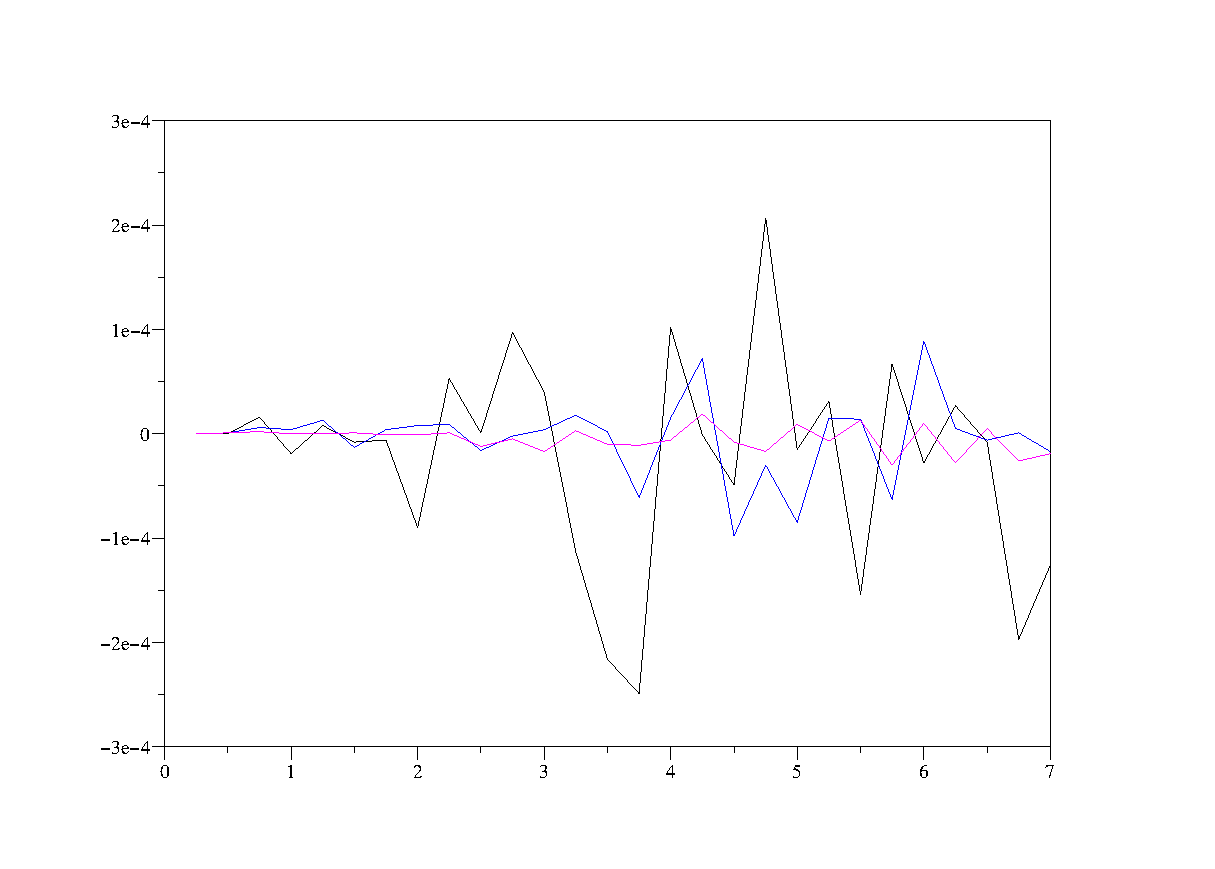
\includegraphics[height=14cm]{./figures/bondserrorY.eps}\\
{\small Computation bonds error with martingale asset Y for $10 000$, $100 000$ and $1 000 000$ Monte-carlo  draws, for $\tau=0.25$ and $M=28$ (Number of factor=$1$, $\gamma_i=0.15$ and $L(0,T_i,T_i)=0.05$)}
\end{center}
%\end{figure}

%\begin{figure}[H]
%\begin{center}
%\includegraphics[height=8cm]{./figures/swptX.eps}
%\caption{Swaption prices w.r.t. the time maturity  expiring at $T=7$
%  computed with $100 000$ Monte-Carlo draws  with martingale asset X.} 
%\label{swptX}
%\end{center}
%\end{figure}

%\begin{figure}[H]
%\begin{center}
%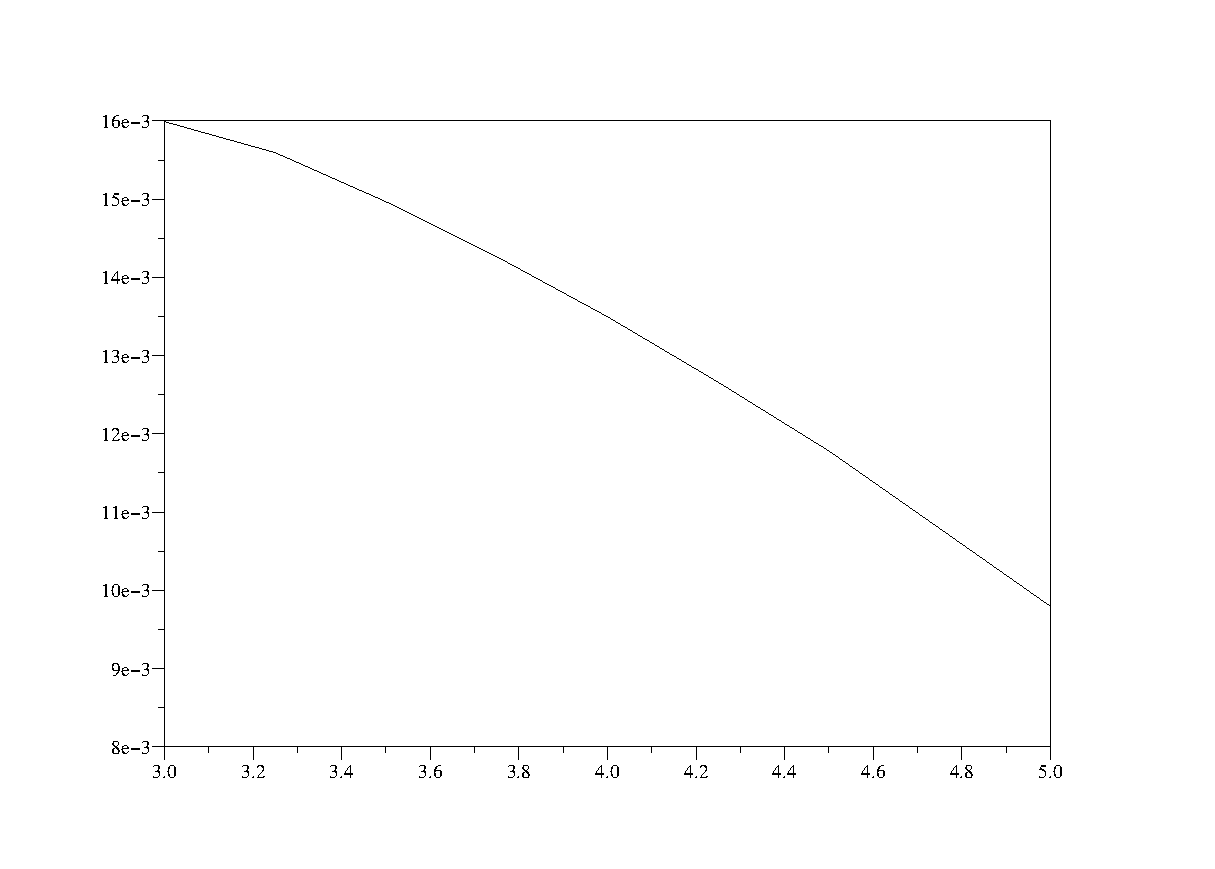
\includegraphics[height=8cm]{./figures/swptY.eps}
%\caption{Swaption prices w.r.t. the time maturity  expiring at $T=7$
%  computed with $100 000$ Monte-Carlo draws  with martingale asset Y.} 
%\label{swptY}
%\end{center}
%\end{figure}

%We can see that the swaption prices simulated with the asset $X$ and the asset $Y$ (for $\tau=0.25$ and $M=28$ Number of factor=$1$, $\gamma_i=0.15$ and 
%$L(0,T_i,T_i)=0.05$) are very similar with a relative precision of $10^{-2}$.



%\section{Bermudan swaption pricing in the Libor Market Model}
 
%\begin{thebibliography}{1}


\begin{thebibliography}{1}

\bibitem{brace1} A. Brace, ``Rank 2 swaption formulae''. Working praper.
 
\bibitem{braceGatarekMusiela} A. Brace, D. Gatarek, M. Musiela, ``The market model of interest rate dynamics'', {\it Mathematical finance}, 7, 127-155.

\bibitem{CLProtter} E.Cl\'ement, D. Lamberton, P.Protter, ``An Analysis of a Least Squares Regression Algorithm for American Option Pricing'', {\it Finance and Stochastic},\textbf{17}, pp. 448-471, 2002

\bibitem{collinDufresneGoldstein} P. Collin Dufresne, R. S. Goldstein, ``Generalizing the affine framework to HJM and random field models'', Working paper.

\bibitem{carrMadan} P. Carr, D. B., Madan, ``Option valuation using fast Fourier tansform'', {\it Journal of Computational Finance}, Vol 2, N$^0$ 4, 61-73, 333.


\bibitem{freeGZ} P. Glasserman and X. Zhao, ``Arbitrage-free discretization of lognormal forward Libor and swap rate models'', {\it Finance and Stochastics} (2000).

\bibitem{LambLap} D. Lamberton, B. Lapeyre, ``Introduction to Stochastic Calculus Applied to Finance'', CRC Press, 1996

\bibitem{Pedersen99} M. B. Pedersen, ``Bermudan Swaptions in the LIBOR Market Model'', {\it SimCorp Financial Research Working Paper}, 1999

\bibitem{Pelsser03} R. Pietersz, A. Pelsser, M. van Regenmortel, ``Fast Drift Approximated Pricing in the BGM Model'', {\emph SSRN Working Paper}, 2004

\bibitem{wuzhang} L. Wu, F. Zhang, ``Libor Market Model : from deterministic to stochastic volatility'', Working paper, 2002




\end{thebibliography}





\end{document}
